\documentclass[mathserif]{beamer}
\usepackage[utf8]{inputenc}
\usepackage{tikz}
\usetheme{Frankfurt}
\usecolortheme{whale}

\title{Calendar Problem 23}
\author{Michael Peng}
\date{The Calendar Month, 2018}
\subtitle{A square with one diagonal as a chord}

\begin{document}
	\frame{\titlepage}
	\begin{frame}
		\frametitle{The Problem}
		Diagonal $AC$ in square $ABCD$ is a
		chord of a circle with radius 12 cm. If $\textrm{m}\widehat{AC} = 30^\circ$, what is the area of $ABCD$?
		
		\begin{center}
		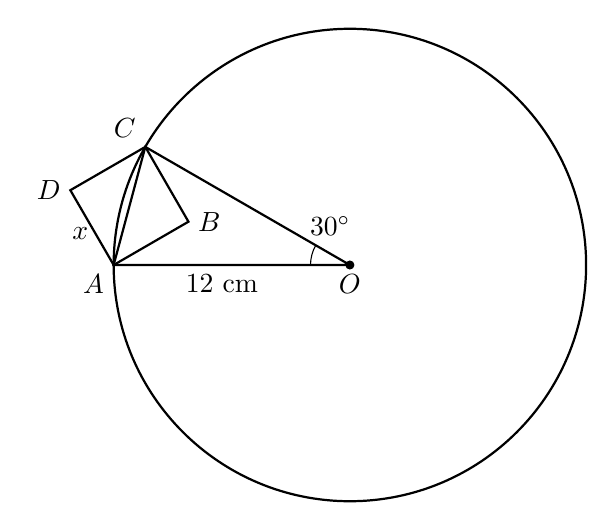
\begin{tikzpicture}[scale=0.25]
			\draw[thick] (0,0) circle [radius=12];
			\draw[fill=black] (0,0) circle [radius=0.2];
			\node[below] at (0,0) {$O$};
			
			\draw[thick] (0,0) -- (-12,0) -- (-10.3923,6) -- cycle;
			\node[below left] at (-12,0) {$A$};
			\node[above left] at (-10.3923,6) {$C$};
			\node[below] at (-6.5,-0) {12 cm};
			\draw (-2,0) arc [radius=2,start angle=180, end angle=150];
			\node[above] at (-1,1) {$30^\circ$};
			
			\draw[thick] (-10.3923,6) -- (-8.2,2.2) -- (-12,0) -- (-14.2,3.8) -- cycle;
			\node[right] at (-8.2,2.2) {$B$};
			\node[left] at (-14.2,3.8) {$D$};
			\node[left] at (-12.8,1.6) {$x$};
		\end{tikzpicture}
		\end{center}
\end{frame}
\begin{frame}
	\frametitle{Finding $AC$}
	\framesubtitle{In the summer...}
	
	\begin{center}
	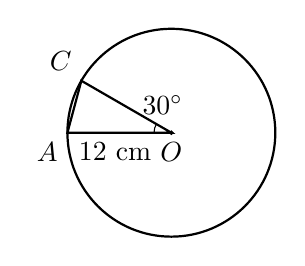
\begin{tikzpicture}[scale=0.11]
	\draw[thick] (0,0) circle [radius=12];
	\draw[fill=black] (0,0) circle [radius=0.2];
	\node[below] at (0,0) {$O$};
	
	\draw[thick] (0,0) -- (-12,0) -- (-10.3923,6) -- cycle;
	\node[below left] at (-12,0) {$A$};
	\node[above left] at (-10.3923,6) {$C$};
	\node[below] at (-6.5,-0) {12 cm};
	\draw (-2,0) arc [radius=2,start angle=180, end angle=150];
	\node[above] at (-1,1) {$30^\circ$};
	\end{tikzpicture}
	\end{center}
		\begin{tabular}{l | l}
			\textrm{m}$\widehat{AC}=30^\circ$ & Given \\
			\textrm{m}$\angle COA=30^\circ$ & Def. of arc measure \\
			$\overline{OA}$ and $\overline{OC}$ are radii of circle $O$ & Def. of radii \\
			$OA=12, OC=12$ & Given \\
			$AC^2=OA^2+OC^2-2(OA)(OC)\cos \angle COA$	& Law of Cosines \\
			$AC^2=12^2+12^2-2(12)(12)\cos 30^\circ$ & Substitution \\
			$AC^2=144+144-288(\frac{\sqrt{3}}{2})$ & Simplification \\
			$AC^2=288-144\sqrt{3}$ & Simplification
		\end{tabular}
\end{frame}
\begin{frame}
	\frametitle{A Square}
	
	\begin{center}
		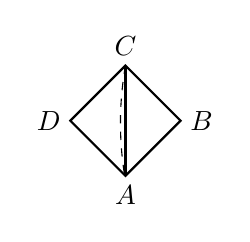
\begin{tikzpicture}[scale=0.7]
		\draw[thick] (0,1) -- (1,0) -- (0,-1) -- (-1,0) -- cycle;
		\draw[thick] (0,1) -- (0,-1);
		\node[above] at (0,1) {$C$};
		\node[below] at (0,-1) {$A$};
		\node[right] at (1,0) {$B$};
		\node[left] at (-1,0) {$D$};
		
		\draw[dashed] (0,1) arc (170:190:6);
		\end{tikzpicture}
	\end{center}
	\begin{tabular}{l | l}
		Quadrilateral $ABCD$ is a square & Given \\
		$ABCD$ has 4 $\cong$ sides and 4 right $\angle$s & Def. of square \\
		$ABCD$ is a rhombus & Def. of rhombuses \\
		$ABCD$ is a rectangle & Def. of rectangles \\
		$[ABCD]=\frac{1}{2}(AC)(BD)$ & Area formula for rhombuses \\
		$\overline{AC}\cong\overline{BD}$ & Diagonals of a rect. are $\cong$ \\
		$AC=BD$ & Definition of segment $\cong$ \\
		$[ABCD]=\frac{1}{2}(AC)(AC)=\frac{1}{2}(AC)^2$ & Substitution
	\end{tabular}
\end{frame}
\begin{frame}
	\frametitle{Finding $[\text{A Square}]$}
	
	\textbf{Deduced: }
		 $[ABCD]=\frac{1}{2}AC^2,AC^2=288-144\sqrt{3}$
	
	\begin{tabular}{l | l}
		$[ABCD]=\frac{1}{2}(288-144\sqrt{3})$ & Substitution \\
		$[ABCD]=\boxed{144-72\sqrt{3}}$ & Simplify
	\end{tabular}
	\vspace{1cm}
	{\huge $$\boxed{144-72\sqrt{3}} \textrm{  cm}^2$$}
\end{frame}
\end{document}